\documentclass[5pt]{article}
%\usepackage{fontspec}
%\setsansfont{Roboto Condensed}
\usepackage{multicol}
\usepackage{calc}
\usepackage{ifthen}
\usepackage[landscape]{geometry}
\usepackage{amsmath,amsthm,amsfonts,amssymb}
\usepackage{color,graphicx,overpic}
\usepackage{hyperref}
\usepackage{gensymb}
\usepackage[sfdefault, condensed]{roboto}
\geometry{top=0.1cm,left=0.1cm,right=0.1cm,bottom=0.2cm}
%I would do the following,
%1. Review the lectures for the theoretical parts (this is the multiple-choice questions)
%2. How the open loop gain and the closed loop gain are linked to each other and which open loop gain you need for a certain accuracy, how to get the gain in dB
%3. Review how to get the transfer functions of amplifiers (inverting, non-inverting amplifiers, superposition principle to be able to get the CMRR, the differential mode gain of amplifiers).  Remember also virtual ground property of amplifiers to simplify much analysis
%4.Sensors types are important (especially resistive, capacitive, and temperature sensors)
%5.DAC types and how to get INL and DNL
%6.Taylor series to approximate functions as I told you in the exercise session

% This sets page margins to .5 inch if using letter paper, and to 1cm
% if using A4 paper. (This probably isn't strictly necessary.)
% If using another size paper, use default 1cm margins.
%\ifthenelse{\lengthtest { \paperwidth = 11in}}
%    { \geometry{top=.5in,left=.5in,right=.5in,bottom=.5in} }
%    {\ifthenelse{ \lengthtest{ \paperwidth = 297mm}}
%        {\geometry{top=1cm,left=1cm,right=1cm,bottom=1cm} }
%        {\geometry{top=1cm,left=1cm,right=1cm,bottom=1cm} } 
%    }

% Turn off header and footer
\pagestyle{empty}

% Redefine section commands to use less space
\makeatletter
\renewcommand{\section}{\@startsection{section}{1}{0mm}%
                                {-1ex plus -.5ex minus -.2ex}%
                                {0.5ex plus .2ex}%x
                                {\normalfont\large\bfseries}}
\renewcommand{\subsection}{\@startsection{subsection}{2}{0mm}%
                                {-1explus -.5ex minus -.2ex}%
                                {0.5ex plus .2ex}%
                                {\normalfont\normalsize\bfseries}}
\renewcommand{\subsubsection}{\@startsection{subsubsection}{3}{0mm}%
                                {-1ex plus -.5ex minus -.2ex}%
                                {1ex plus .2ex}%
                                {\normalfont\small\bfseries}}
\makeatother

% Define BibTeX command
\def\BibTeX{{\rm B\kern-.05em{\sc i\kern-.025em b}\kern-.08em
    T\kern-.1667em\lower.7ex\hbox{E}\kern-.125emX}}

% Don't print section numbers
\setcounter{secnumdepth}{0}


\setlength{\parindent}{0pt}
\setlength{\parskip}{0pt plus 0.5ex}

%My Environments
\newtheorem{example}[section]{Example}
% -----------------------------------------------------------------------

\begin{document}
\raggedright
\footnotesize
\begin{multicols*}{4}


% multicol parameters
% These lengths are set only within the two main columns
%\setlength{\columnseprule}{0.25pt}
\setlength{\premulticols}{1pt}
\setlength{\postmulticols}{1pt}
\setlength{\multicolsep}{1pt}
\setlength{\columnsep}{2pt}

\begin{center}
     \Large{\underline{TMS II}} \\
 
\end{center}


% Summary starts here
% --------------------------------------------------------------------------------------
\subsection{Begriffsdefinitionen}
\subsubsection{Konfigurationsmanagement}
KM stellt sicher, dass Produkte eindeutig identifizierbar sind, Zusammenhänge und Unterschiede von
verschiedenen Versionen einer Konfiguration erkennbar bleiben und Produktänderungen nur kontrolliert durchgeführt werden können.
Arten der Durchführung:
- Automatisch (z.B. Git)\\
- Manuell\\
- Semi-automatisch (z.B. unterstützende Plugins)\\
\textbf{Build-Management}\\
Unter Build-Management wird diejenige Funktion verstanden, die alle Bauteile einer Konfiguration
erzeugt, die nicht direkt vom Benutzer erstellt oder durch das System vorgegeben wurden. Zentrale Fragen: Wie ist die Software zusammengestellt? Welche Abhängigkeiten müssen berücksichtigt werden? Beispiele für klassische Abhängigkeiten:
o Entwicklungsumgebung: Editor, Generatoren, Compiler, Linker, …\\
o Basissoftware: LAN, ...\\
o Betriebssystem\\
o Hardware\\
\textbf{Change-Management}\\
Im Änderungswesen muss definiert werden, wie Änderungswünsche (Change Requests) erfasst
werden, wie und durch wen diese bewertet werden und wie die Durchführung von Änderungen
zu erfolgen hat.\\
- Versions-Management (Wer hat wann was geändert?)
Versionsmanagement befasst sich (in erster Linie mit der Verwaltung der zeitlich aufeinander folgenden Revisionen eines Dokuments.)
\textbf{Release-Management}\\
Ein Release ist eine an Kunden ausgelieferte Konfiguration eines (Software-)Systems, bestehend
aus ausführbaren Programmen, Bibliotheken, Dokumentation, Quelltexten, Installationsskripten
und so weiter. Das Release-Managementdokumentiert ausgelieferte Konfigurationen und stellt
deren Rekonstruierbarkeit sicher.
Geplant
\subsubsection{Produktzustände}
\textbf{In Bearbeitung}\\
Das Produkt wird bearbeitet. Es befindet sich entweder im privaten Entwicklungsbereich des
Entwicklers oder unter Kontrolle des Entwicklers innerhalb der Produktbibliothek.\\
\textbf{Vorgelegt}\\
Das Produkt ist aus der Sicht des Erstellers fertig und wird der Konfigurationsverwaltung übergeben. Ab jetzt kann es einer Prüfung durch die Qualitätssicherung unterzogen werden. Wird das
Produkt hierbei abgelehnt, so geht es wieder in den Zustand in Bearb. zurück, andernfalls rückt
es in den Zustand akzeptiert vor. Ab dem Zustand vorgelegt an kann der Ersteller nur unter
Fortschreibung der Versionsangabe Modifikationen durchführen.\\
\textbf{Akzeptiert}\\
Das Produkt wurde durch die QS überprüft und freigegeben. Es darf nur noch innerhalb einer
neuen Version geändert werden.
\columnbreak
\subsection{CTL}
\subsubsection{Pfadoperatoren:}
- $A \phi$ - auf allen Pfaden folgt $\phi$ (englisch: AIl) \\ 
- E $\phi$ - auf mindestens einem Pfad folgt $\phi$ (englisch: Exists) \\ 
\subsubsection{Pfad-spezifische Operatoren:}
- $X \phi$ - unmittelbar folgt $\phi$ (englisch: neXt state) \\ 
- $F \phi$-irgendwann folgt $\phi$ (englisch: some Future state oder Finally) \\ 
- $G \phi$ - auf dem folgenden Pfad folgt in jedem Zustand $\phi$ (englisch: Globally) \\ 
- $\phi U \psi-\phi$ folgt bis zum Erreichen des Zustands $\psi$ (englisch: Until) \\ 
- $\phi W \psi-\phi$ folgt immer oder bis zum Erreichen des Zustands $\psi$ (englisch: Weak Until) \\ 
- $E X \phi$ - in (mind.) einem nächsten Zustand gilt $\phi$ \\ 
- $E F \phi$ - in (mind.) einem der folgenden Zustände gilt $\phi$ \\ 
- EG $\phi$ - es gibt (mind.) einen Pfad, so dass $\phi$ entlang des ganzen Pfades gilt \\ 
- $E[\phi U \psi]$ - es gibt einen Pfad, für den gilt: bis zum ersten Auftreten von $\psi$ gilt $\phi$ \\ 
- $A X \phi$ - in jedem nächsten Zustand gilt $\phi$ \\ 
- AF $\phi$ - man erreicht immer einen Zustand, in dem $\phi$ gilt \\ 
- $A G \phi$ - auf allen Pfaden gilt in jedem Zustand $\phi$ \\ 
- $A[\phi U \psi]$ - es gilt immer $\phi$ bis zum ersten Auftreten von $\psi$ \\ 
\subsubsection{Semantik}
- $T\left(s_0\right) \models \neg \phi \quad \Leftrightarrow \quad T\left(s_0\right) \not \models \phi$ \\ 
- $T\left(s_0\right) \models \phi \vee \psi \quad \Leftrightarrow \quad T\left(s_0\right) \models \phi \operatorname{oder} T\left(s_0\right) \models \psi$ \\ 
- $T\left(s_0\right) \models E X \phi \quad \Leftrightarrow \quad T\left(s_1\right) \models \phi$ \\ 
- $T\left(s_0\right) \models E G \phi \quad \Leftrightarrow \quad \forall i: T\left(s_i\right) \models \phi$ \\ 
- $T\left(s_0\right) \models \phi E U \psi \quad \Leftrightarrow \quad \exists k: T\left(s_k\right) \models \psi \wedge \forall i<k: T\left(s_i\right) \models \phi$ \\ 
\subsubsection{Transformationen} 
- $\neg A \phi \equiv E \neg \phi$ \\ 
- $\neg A F \phi \equiv E G \neg \phi$ \\ 
- $\neg E F \phi \equiv A G \neg \phi$ \\ 
- $\neg A X \phi \equiv E X \neg \phi$ \\ 
- $A G \phi \equiv \phi \wedge A X A G \phi$ \\ 
- $E G \phi \equiv \phi \wedge E X E G \phi$ \\ 
- $A F \phi \equiv \phi \vee A X A F \phi$ \\ 
- $E F \phi \equiv \phi \vee E X E F \phi$ \\ 
- $A[\phi U \psi] \equiv \psi \vee(\phi \wedge A X A[\phi U \psi])$ \\ 
- $E[\phi U \psi] \equiv \psi \vee(\phi \wedge E X E[\phi U \psi])$
\subsection{Wahrheitstabelle}
$    \begin{array}{|c c|c|c|c|}

    p & q & p \land q & p\lor q  & p \rightarrow q  \\ 
    \hline % Put a horizontal line between the table header and the rest.
    T & T & T& T& T\\
    T & F & F& T& F\\
    F & T & F& T& T\\
    F & F & F& F& T\\
    \end{array}
 $
\section{Aufwandsschätzung}
% \textbf{Wenn Entwicklung und Wartung in Aufgabentext getrennt gilt Integal nicht Exponentialformeln. für $N_W$ wird mit $k$ multipliziert. $N_e $}
\subsection{Entwicklungsleistung bekannt}
\textbf{Gesamtleistung} $N_G(t)=f(t)+k \cdot \int f(t) \cdot d t+C$\\
\textbf{Wartungsleistung} $N_W(t)=k \cdot \int f(t) \cdot d t+C$\\
\textbf{Entwicklungsleistung} $N_E(t) = f(t)$\\
\textbf{Gesamtarbeit} $A_G(t)=A_E(t)+A_W(t)$\\
\textbf{Entwicklungsarbeit} $A_E(t)=\int f(t) \cdot d t+C$\\
\textbf{Wartungsarbeit} $A_W(t)=k \cdot \int\left[\int f(t) \cdot d t+C_1\right] \cdot d t+C_2$\\

\subsection{Gesamtleistung bekannt}
% TODO 3 fälle auf den Folien mitschrieb 4
\textbf{Gesamtleistung} $g(t)=N_g= [Mann]$ Anzahl Leute \\
\textbf{Wartungsleistung} $N_W(t)=k \cdot e^{-k t}\left[\int e^{k t} \cdot g(t) d t+C\right] \stackrel{C=0}{=} k \cdot e^{-k t} \cdot N_G \cdot \int_0^t e^{k t} d t=N_G\left(1-e^{-k t}\right)$\\
\textbf{Entwicklungsleistung} $N_E(t)=N_G-N_W(t)=N_G \cdot e^{-k t}$
\textbf{Gesamtarbeit} $A_G= N_G \cdot t$\\
\textbf{Entwicklungsarbeit} $ A_E(t)=\frac{1}{k} \cdot N_G\left(1-e^{-k t}\right)$\\
\textbf{Wartungsarbeit} $A_W(t)=A_G(t)-A_E(t)=N_G \cdot t-A_E(t)=N_G\left[t-\frac{1}{k} \cdot\left(1-e^{-k t}\right)\right]$\\
\subsection{Entwicklungsarbeit bekannt}
\textbf{Gesamtleistung} $N_G(t) = N_E(t) + N_W(t)$\\
\textbf{Wartungsleistung} $N_W(t)=k \cdot h(t)+C$\\
\textbf{Entwicklungsleistung} $N_E(t)=\frac{d h(t)}{d t}$\\
\textbf{Gesamtarbeit} $A_G(t)=h(t)+A_W(t)$\\
\textbf{Entwicklungsarbeit} $A_E(t) = h(t)$\\
\textbf{Wartungsarbeit} $A_W(t)=\int[k \cdot h(t)+C] \cdot d t+C_1$
mit $k=\left[ \dfrac{Mann}{Mannjahr}\right]$ Wartungsintensität\\
\section{Reverse Engineering}
\subsection{Structure Chart}
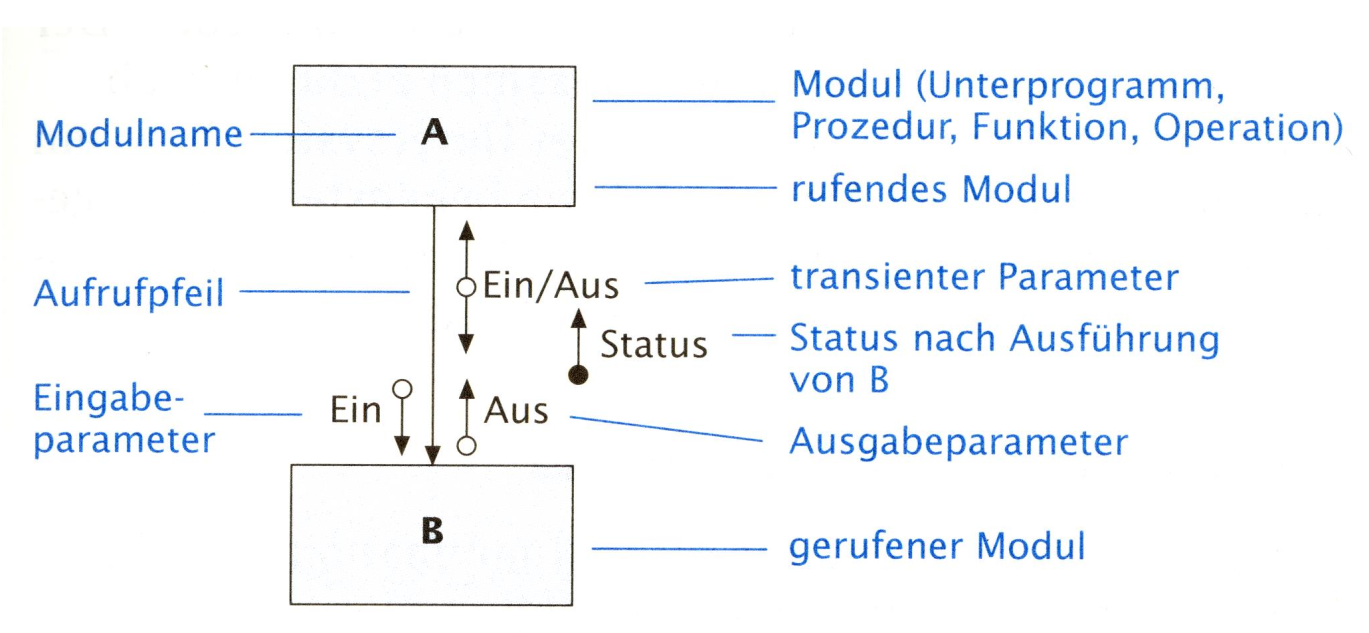
\includegraphics[width= \columnwidth]{images/structureChart.png}\\
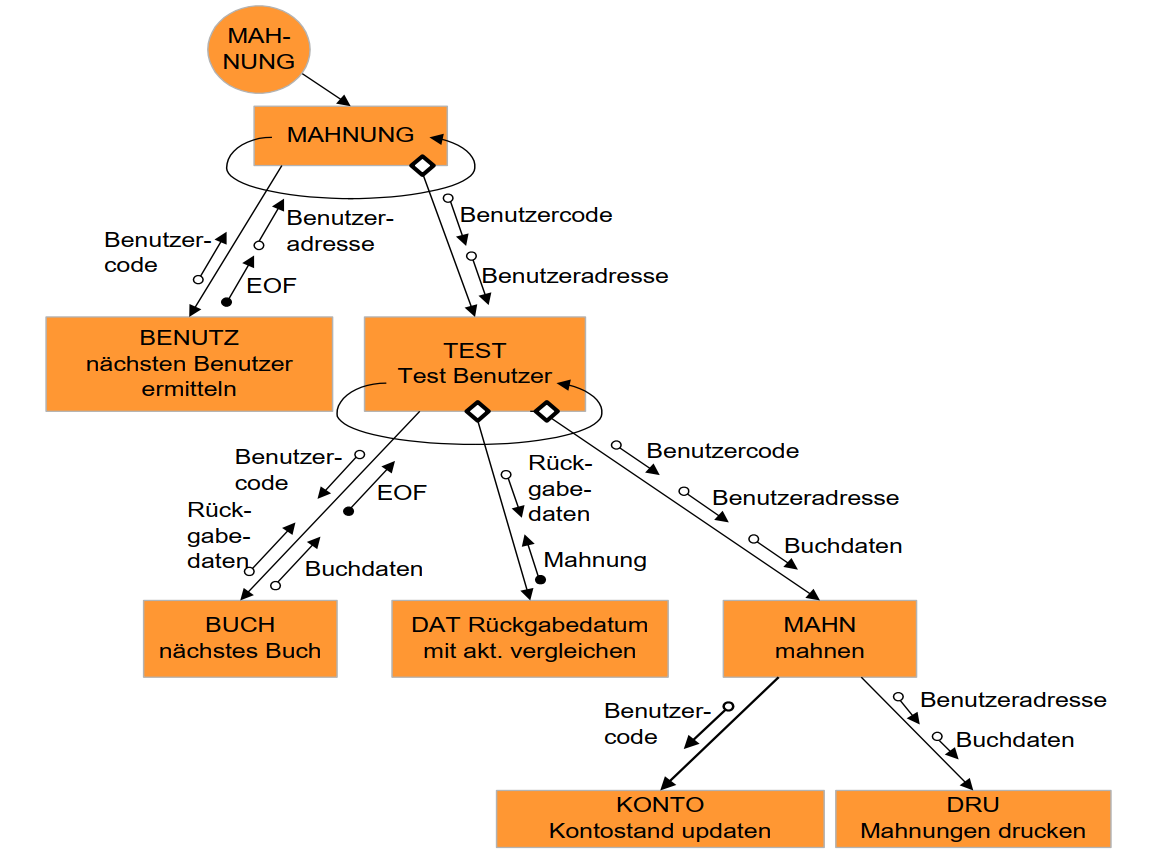
\includegraphics[width= \columnwidth]{images/bspStructChart.png}\\
\subsection{Nesting tree}
Indent tree \\
TODO Maybe add picture\\
\section{Datenbanken}
\subsection{Normalformen}
\subsubsection{1. Normalform}
Jedem Datenfeld eines Datensatzes darf höchstens ein Wert
zugewiesen sein. D.h. es dürfen keine Mehrfacheinträge in einem Datenfeld vorliegen und Attribute müssen atomar sein.
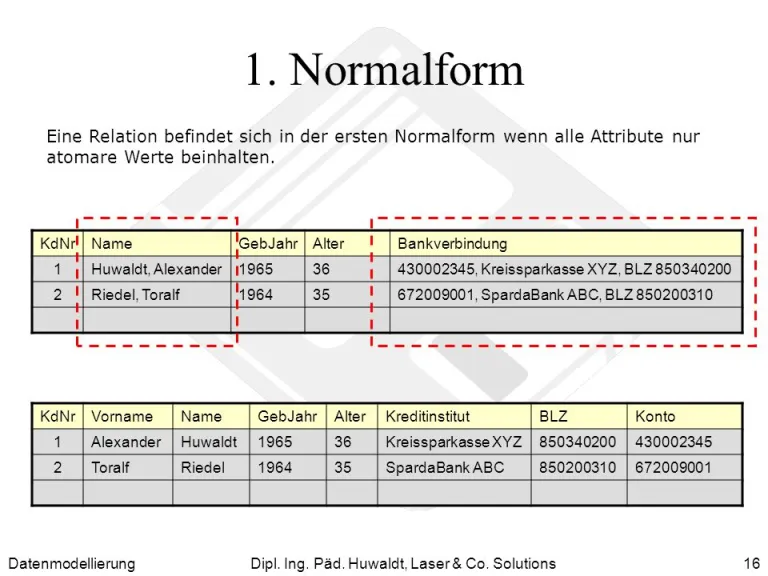
\includegraphics[width = \columnwidth]{images/1normalformEx.png}
\subsubsection{2. Normalform}
Erfüllt 1. Normalform \\
Eine Tabelle enthält nur Daten eines Themen- bzw. Informationsbereiches.\\
Aufteilung in mehrere Tabellen nach Themen/ Informationsgebieten.\\
Jedes Nicht-Schlüsselfeld  muss durch ein Schlüsselfeld identifizierbar sein und vom gesamten Schlüssel abhängen.\\
Überprüfen und ggf. neue Schlüsselfelder hinzufügen oder zusammengesetzte Schlüssel definieren.\\
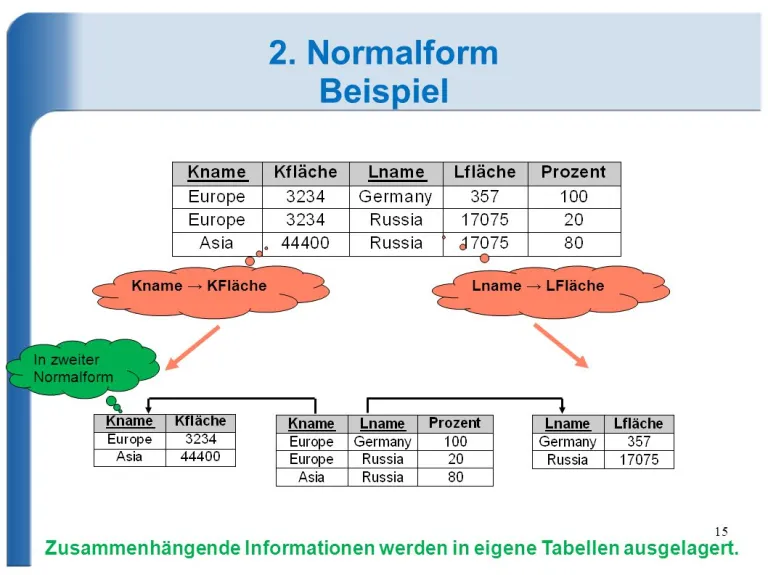
\includegraphics[width = \columnwidth]{images/2normalformEx.png}
\subsubsection{3. Normalform}
Ist dann erfüllt, wenn die Tabelle die 2. Normalform erfüllt\\
Es dürfen keine transitiven (indirekten) Abhängigkeiten vorliegen.\\
Entfernung aller transitiven Abhängigkeiten durch Aufspalten der Tabelle in mehrere Tabellen, in denen alle Nicht-Schlüsselfelder direkt vom gesamten Schlüsselfeld abhängen\\
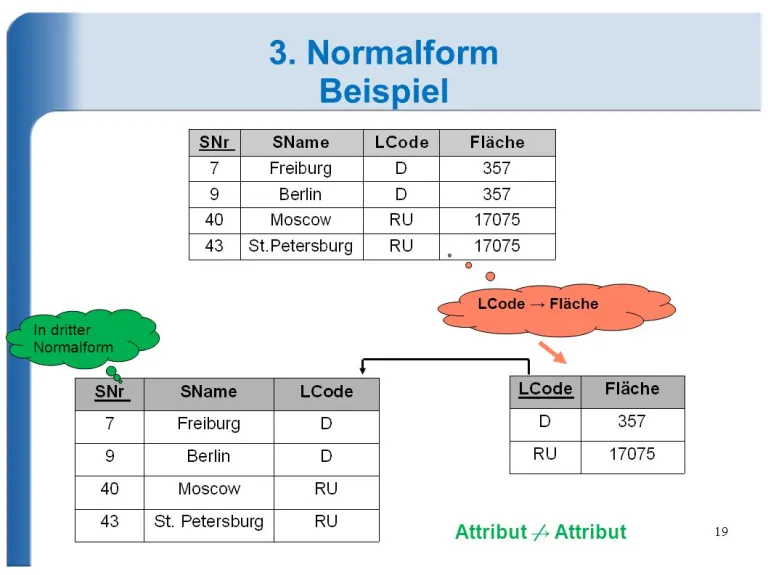
\includegraphics[width = \columnwidth]{images/3normalformEx.png}
\section{ERD}
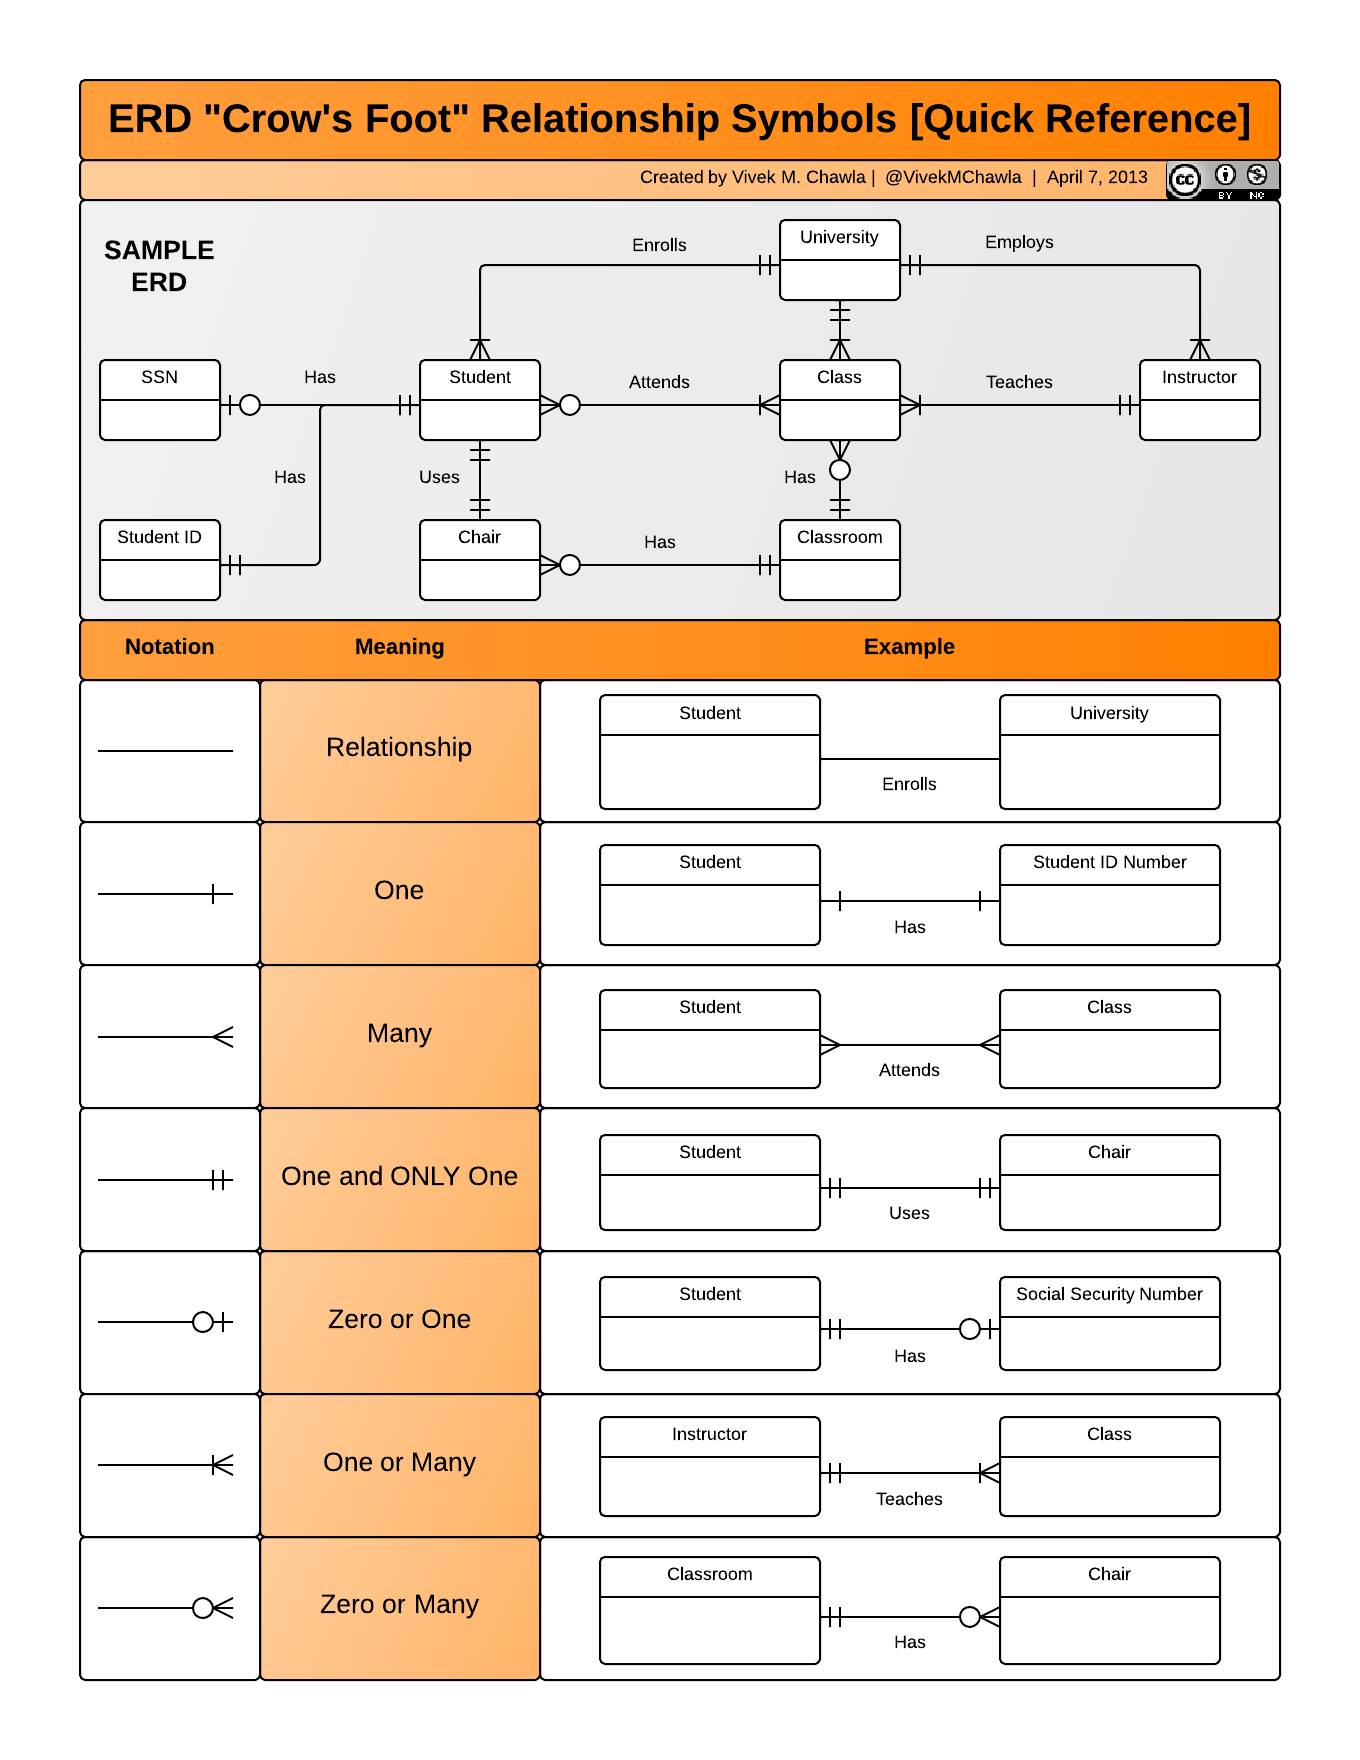
\includegraphics[width = \columnwidth]{images/5uwcF.png}\\
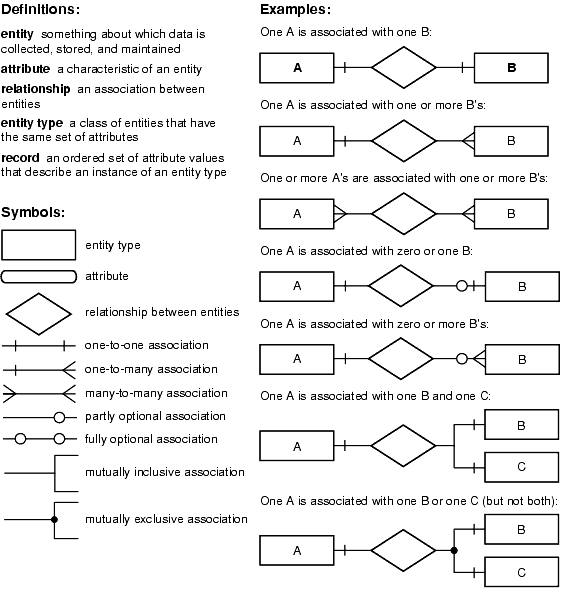
\includegraphics[width = \columnwidth]{images/9tvIZ.png}\\
\section{GAIA}
\subsection{Role Model Template}
\begin{tabular}{|l|l|}
    \hline
    Role Schema:&\\
    \hline
    Description:&\\
    \hline
    Protocols and \underline{Activities}: & \\
    \hline
    Permissions:  & - reads:\\
    & - changes:\\
    & - generates:\\
    \hline
    Responsibilities: & - Liveness:\\
    & - Safety:\\
    \hline
\end{tabular}\\
\subsection{Template for Interaction Model}
\begin{tabular}{|c|c|}
    \hline
    [Protocol's name]  &[Inputs]\\
    \hline
    [Initiator] \quad \vline  \quad [Responder] & \\
    \hline
    [Description] & [Outputs] \\
    \hline
\end{tabular}
\begin{itemize}
    \item Description: Beschreibung
    \item Initiator: Rolle
    \item Responder: Rolle
    \item Inputs: Informationen des Auslösers
    \item Outputs: Informationen des Beantworters
\end{itemize}
\subsection{Operatoren Ablaufbeschreibung}
\begin{tabular}{ll}
    Operator & Interpretation\\
    $x . y$ & x followed by y\\
    $x|y  $ & x or y occurs\\
    $x^* $ & x occurs 0 or more times\\
    $X+$  & x occurs 1 or more times\\
    $x^{\omega}$ & x occurs innately often\\
    $\left[x\right]$ & x is optional\\
    $ x || y $ & x and y are interleaved(verschachtelt)
\end{tabular}
\subsection{Service Model}
\begin{tabular}{|c|c|c|c|c|}
    \hline
    Service & Inputs & Outputs & Precondition& Post-condition \\
    \hline
    &&&&\\
    \hline    
\end{tabular}
%  Nesting tree and Structure chart, empty circle is data flow full circle is control flow folien ue5
% TODO ER Diagramme cheat sheet
% TODO Revisit ex8 last task
\end{multicols*}
\end{document}






























 